\subsection{Third party libraries that process the input data to the system}
\label{ros_packages}
In this section the ROS packages that are used in our system are presented. 
All of them are used for the initial processing of the data coming from the RGB-D sensor. 
The connection between them and the developed nodes are explained in this section and in section \ref{nodes}.

\paragraph{ROS package: openni\_camera}\mbox{} \\
\label{openni_camera}

This packages implements the RGB-D sensors drivers.
% It is needed to connect the kinect to the computer. 
% The package is composed of nodes that perform different tasks and publish the results in topics. 
% As an example, a node transforms the raw output information of the kinect into a data array for further processing. 
The package transforms the input raw data coming from the kinect into structured one. 
This information is prepared hence for further processing. 
Figure \ref{diagram_kinect_data} shows the inputs and outputs of this package and its position in the RGB-D sensor data processing chain. 
 
 		\begin{figure}[H]
			\begin{center}
			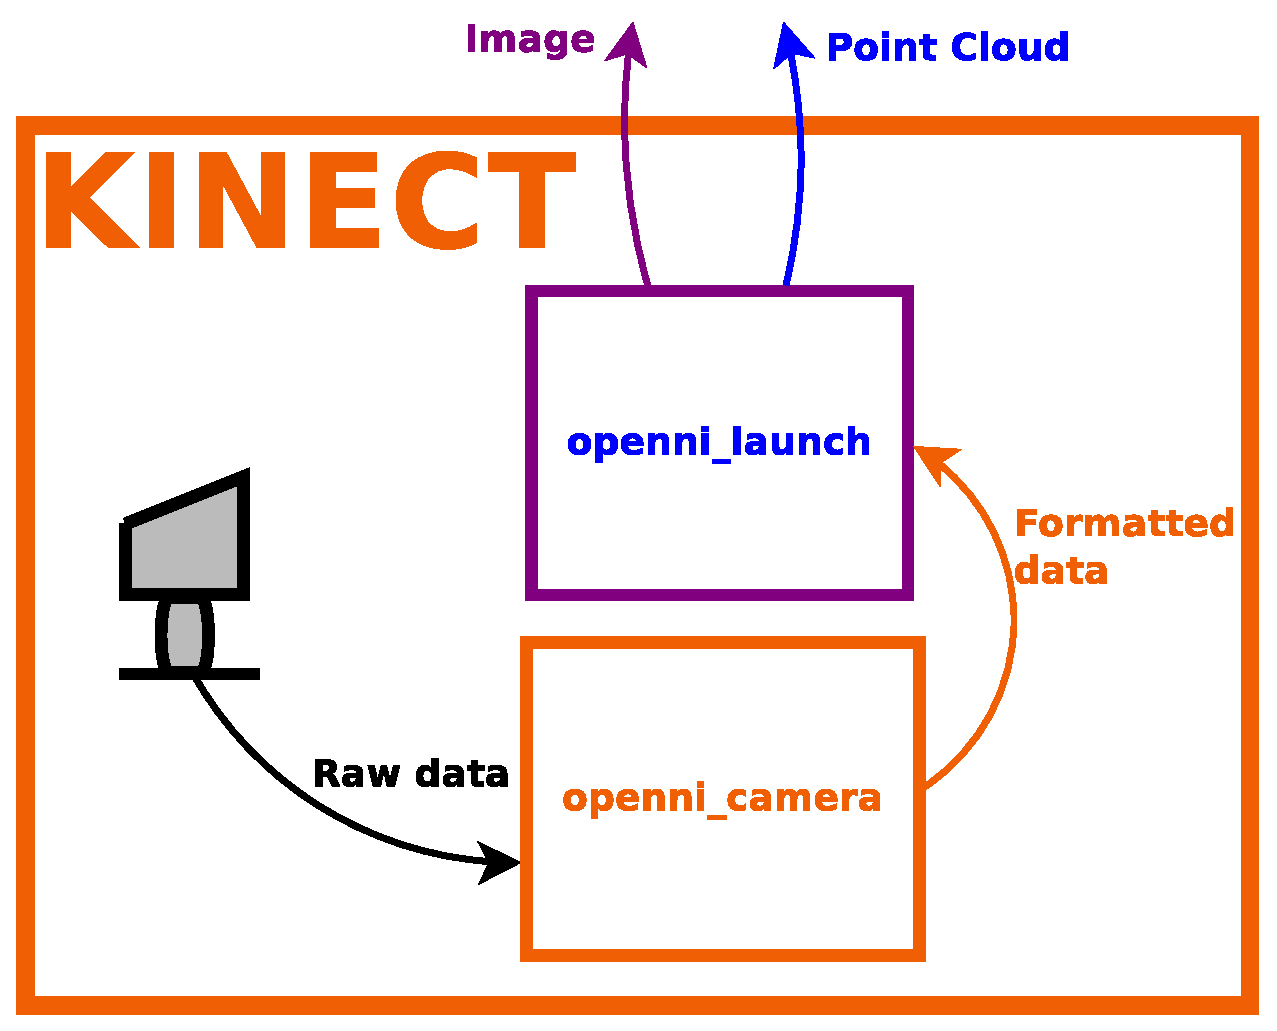
\includegraphics[width=0.5\linewidth]{img/diagrams/kinect_data.eps}
			\caption[Kinect data processing]{Kinect data processing using the openni ROS packages (openni\_camera and openni\_launch).}
			\label{diagram_kinect_data}
			\end{center}
		\end{figure}


\paragraph{ROS package: openni\_launch}\mbox{}\\
\label{openni_launch}

This package provide useful transformations taking as input the openni\_camera topics. %and a launch file that executes nodelets with that information. 
It is composed of various nodes that can be executed using a launch file. 
Each node processes the raw input information from the driver into more complicated and useful data. 
That data may be a registered point cloud or a disparity image for example. 
The output of the nodes is published into different topics. 
The developed nodes described in section \ref{nodes} are subscribed to these topics in order to obtain the input point cloud and image. 



\paragraph{ROS package: pi\_tracker}\mbox{}\\

This ROS package implements a joint tracker.
It is used within the system to determine the position and orientation of the user's joints. 
This task is performed by the skeleton tracker node.  
Figure \ref{diagram_skeleton} shows the inputs and outputs of this node. 
The diagram presented in figure \ref{diagram_kinect_data} is simplified in the next figures.  

		\begin{figure}[H]
			\begin{center}
			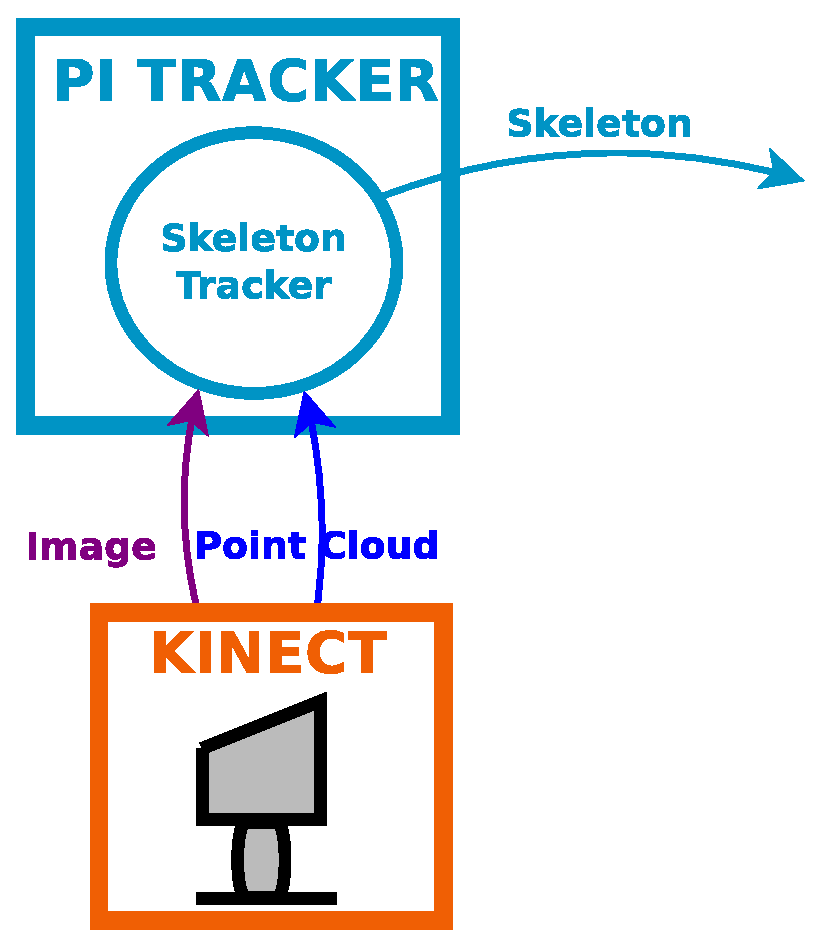
\includegraphics[width=0.3\linewidth]{img/diagrams/node_pi_tracker.eps}
			\caption[Skeleton Tracker I/O]{Inputs and outputs of the Skeleton Tracker node.}
			\label{diagram_skeleton}
			\end{center}
		\end{figure}

It can be seen that the node takes as input the output data of the openni\_launch ROS package. 
The node outputs the Skeleton message in which the positions and orientations of the joints are represented. 



\newpage
%%%%%%% SOFTWARE NODES %%%%%%
%\addcontentsline{toc}{subsection}{Software nodes}
\subsection{Developed nodes}
\label{nodes}


The processing needed to provide all the functionality is divided in nodes. 
Here they are presented, ordered using the data work-flow. 
First the ones using the raw input data to the system and afterwards the ones that deliver the output of the system are described.
Figure \ref{system_nodes} shows a node diagram. 
The circles represent the nodes. %Each circle is a node and the name inside them is the one being used in the software. 
The arrows show the communication between nodes. 
The names next to the lines are the messages that those processes interchange. 
The squares with the names serve as separators of the different packages that are being used. 
All the nodes inside the square with the title "OCULAR" are the ones I developed. 
In the following sections the processing performed by each node is presented. 
\\


		\begin{figure}[H]
			\begin{center}
		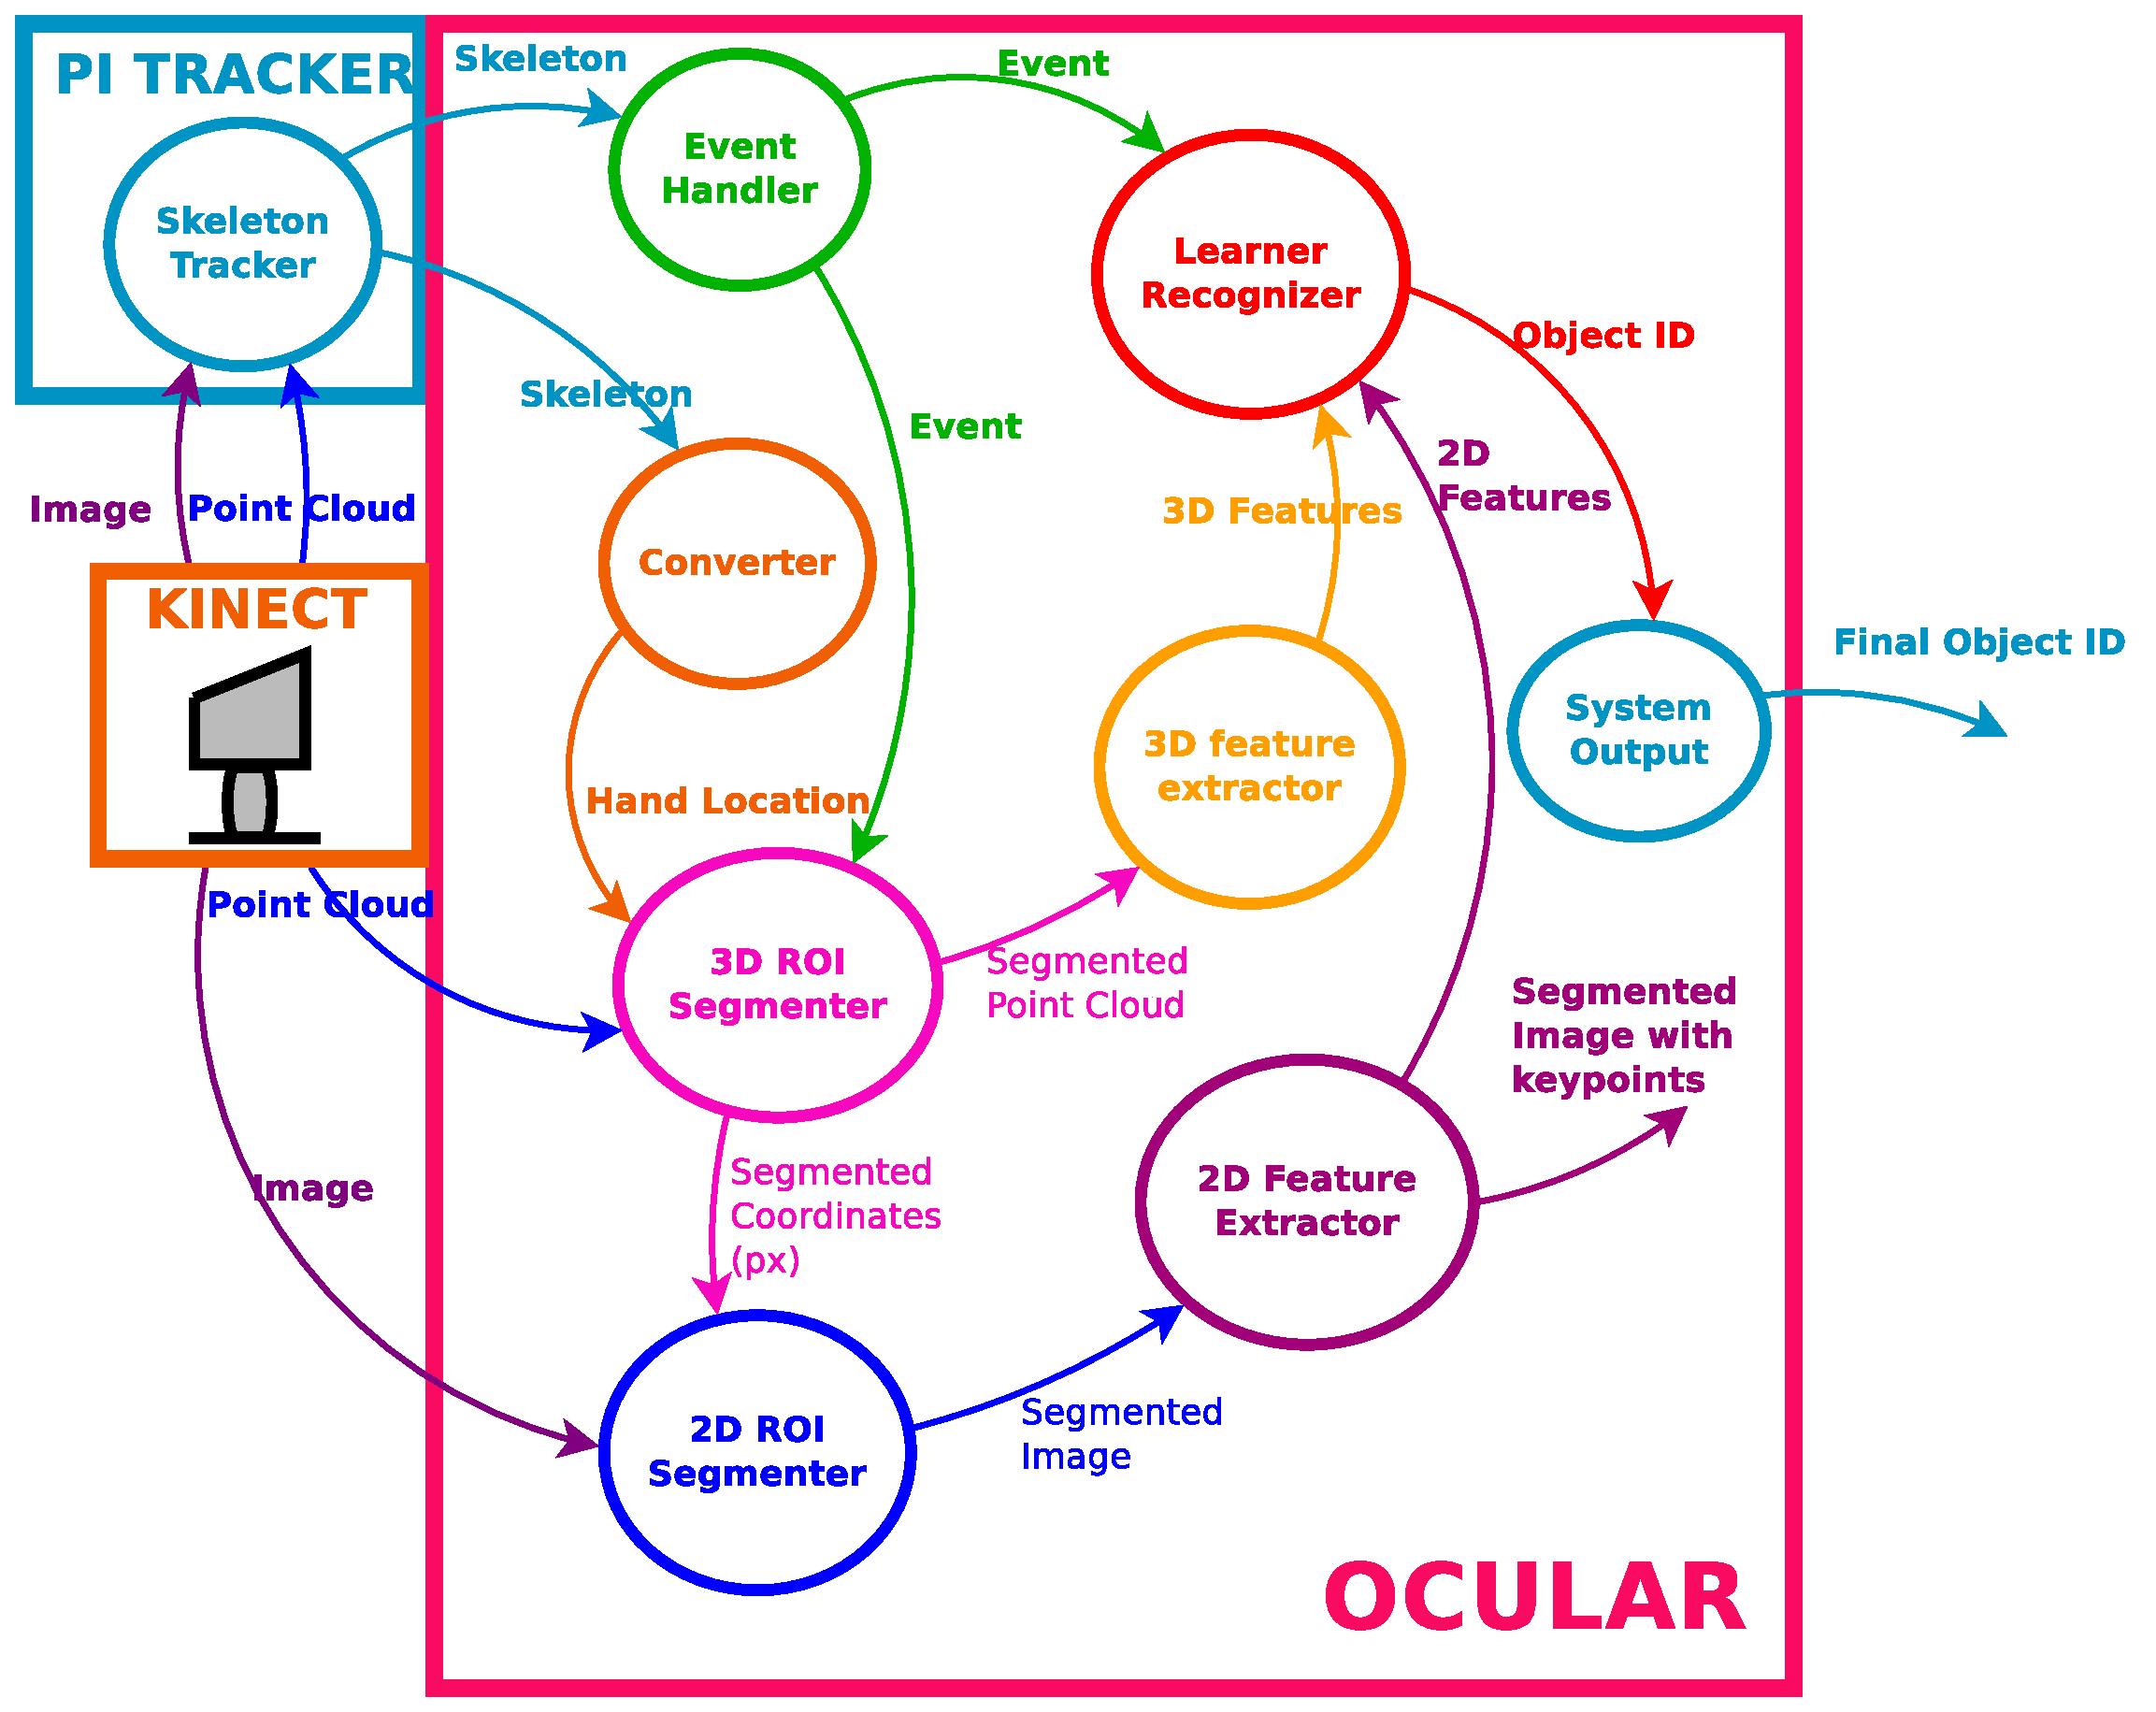
\includegraphics[width=\linewidth]{img/diagrams/nodes.eps}
			\caption[System nodes]{System nodes and their interaction.}
			\end{center}
			\label{system_nodes}
		\end{figure}

\newpage



%\newpage


\paragraph{Converter}\mbox{}\\
		\label{converter}

	This node is the first step of the developed software. 
	It transforms the input data from the pi\_tracker package into the custom message used within the software. 
	Figure \ref{node_converter} represents the inputs and outputs of the node. 
	The skeleton message enters the node and the custom message containing the hands location is the output. 

		\begin{figure}[H]
			\begin{center}
			\includegraphics[width=0.5\linewidth]{img/diagrams/node_converter.png}
			\caption[Converter node I/O]{Inputs and outputs of the Converter node.}		
			\label{node_converter}
			\end{center}
		\end{figure}

	% The information provided by that third-party code contains the position in the space of each joint of the body. 
	% The converter node takes only both hand's position. 
	The use case diagram of the node can be seen in figure \ref{uc_converter}. 

	\begin{figure}[H]
		\centering
		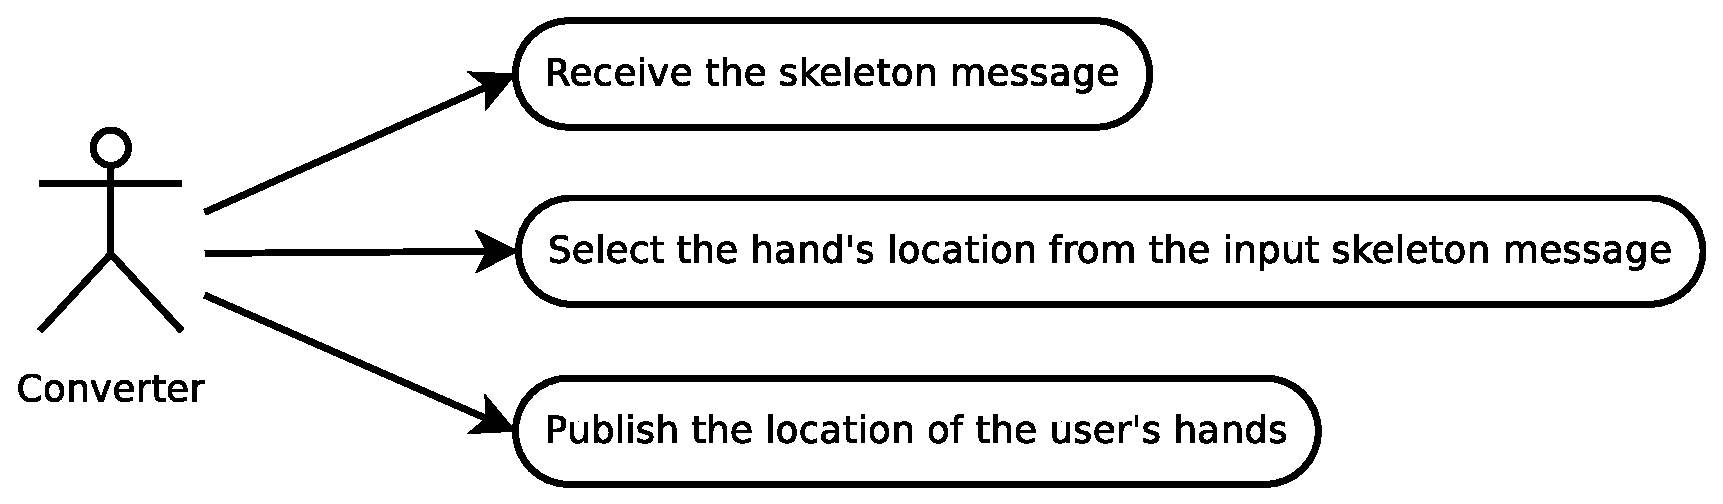
\includegraphics[scale=0.4]{img/diagrams/uc_converter.eps}
		\caption[Use case diagram converter node]{Use Case diagram of the converter node}
		\label{uc_converter}
	\end{figure}

	
	%\newpage

\paragraph{ROI Segmenter 3D}\mbox{}\\
	\label{roi_segmenter_3d}

	Figure  \ref{node_roi3d} presents the inputs and outputs of the node. 
	The input of this node is the raw 3D information from the sensor and the hand's locations from the third-party package pi\_tracker, as well as the hand in which the user is holding the object. 

		\begin{figure}[H]
			\begin{center}
			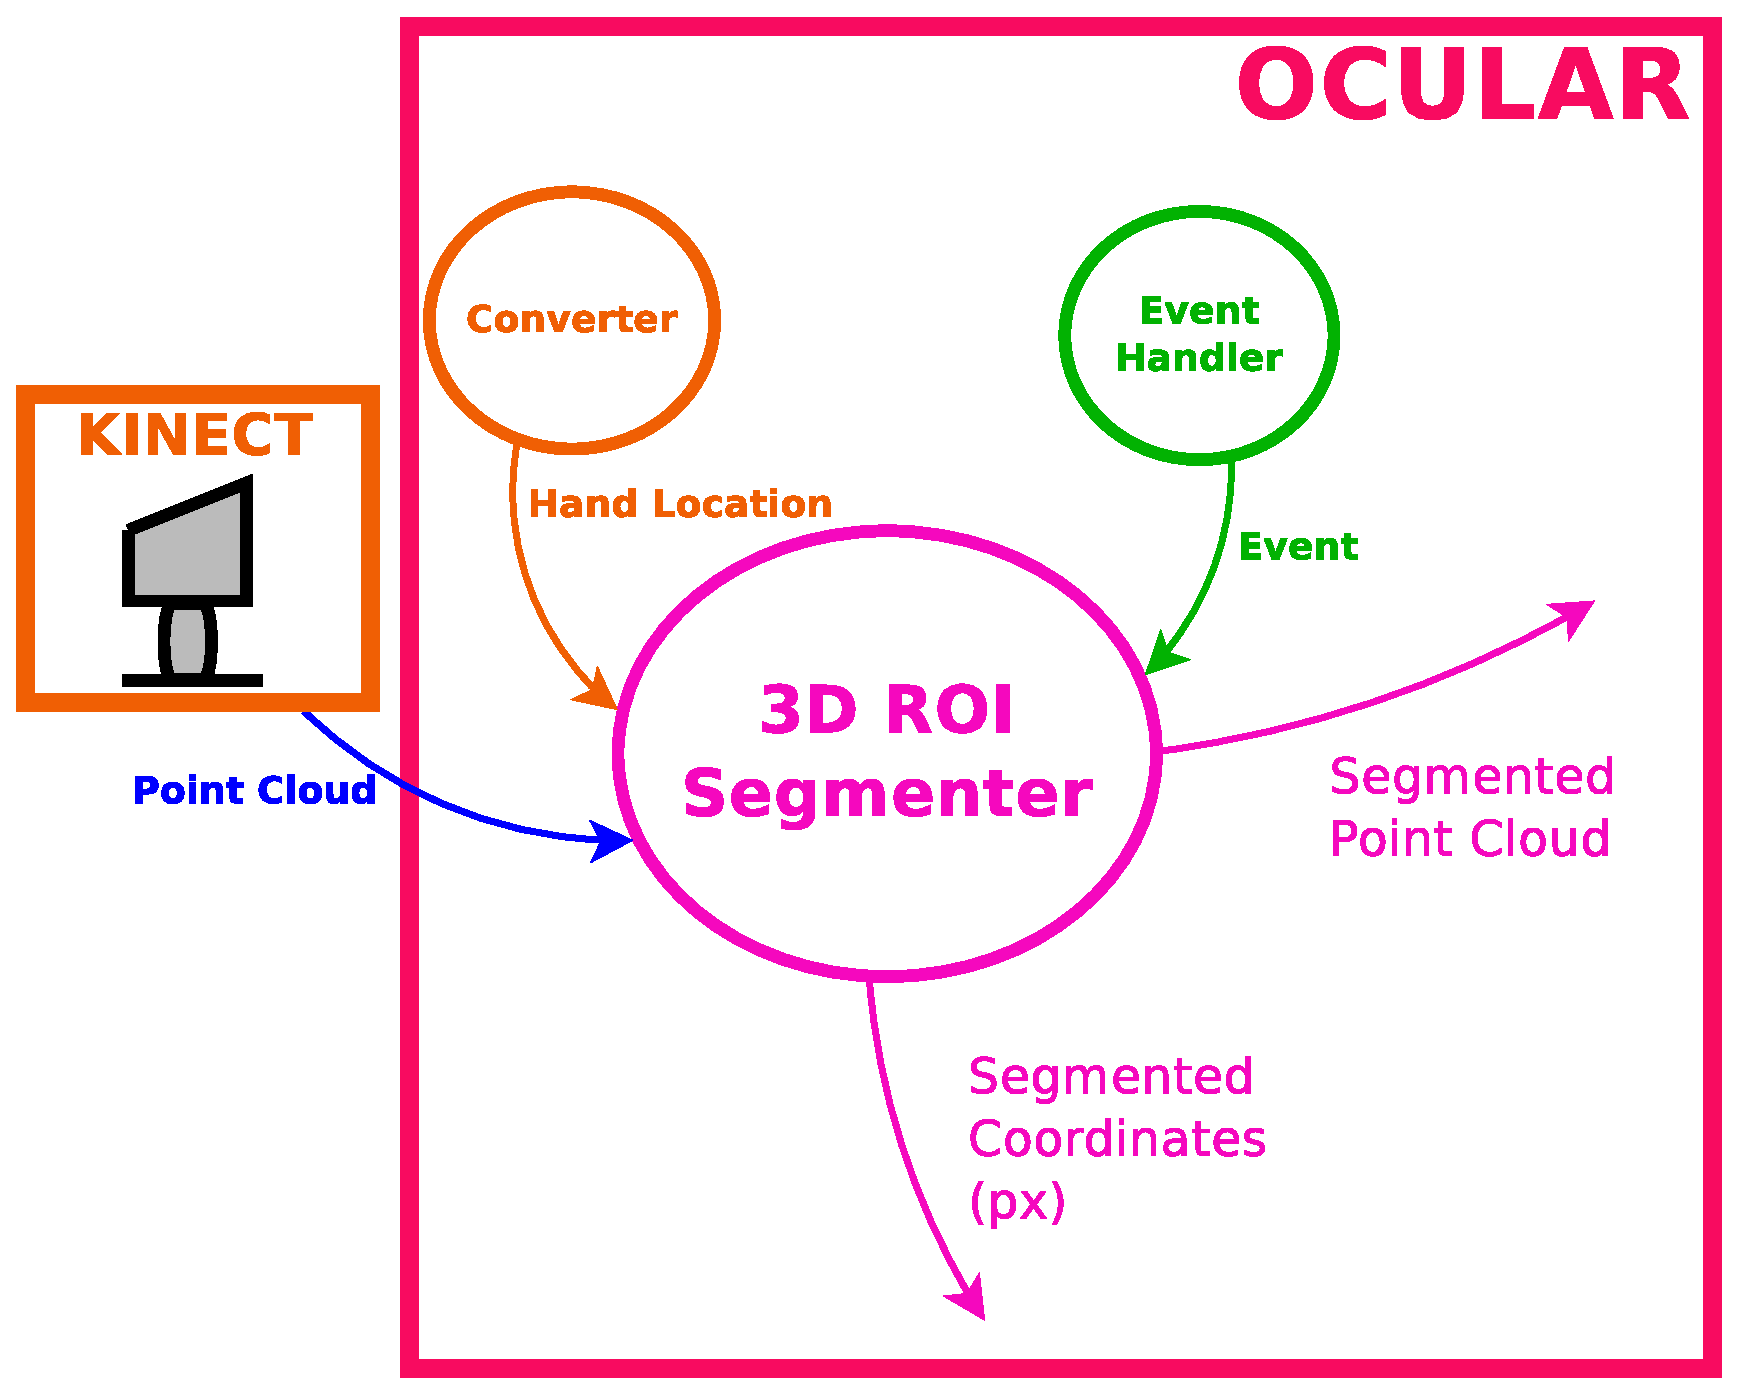
\includegraphics[width=0.5\linewidth]{img/diagrams/node_roi3d.eps}
			\caption[ROI segmenter 3D node I/O]{Inputs and outputs of the ROI segmenter 3D node.}		
			\label{node_roi3d}
			\end{center}
		\end{figure}


	The node segments a prism from the original point cloud around the selected hand's center. 
	The prism vertex coordinates are transformed from world coordinates to pixels. 
	This is done to allow the ROI Segmenter 2D to perform the cropping of the input image using those pixel values. 
	That information is the output of the node, together with the segmented point cloud. 

	\begin{figure}[H]
		\centering
	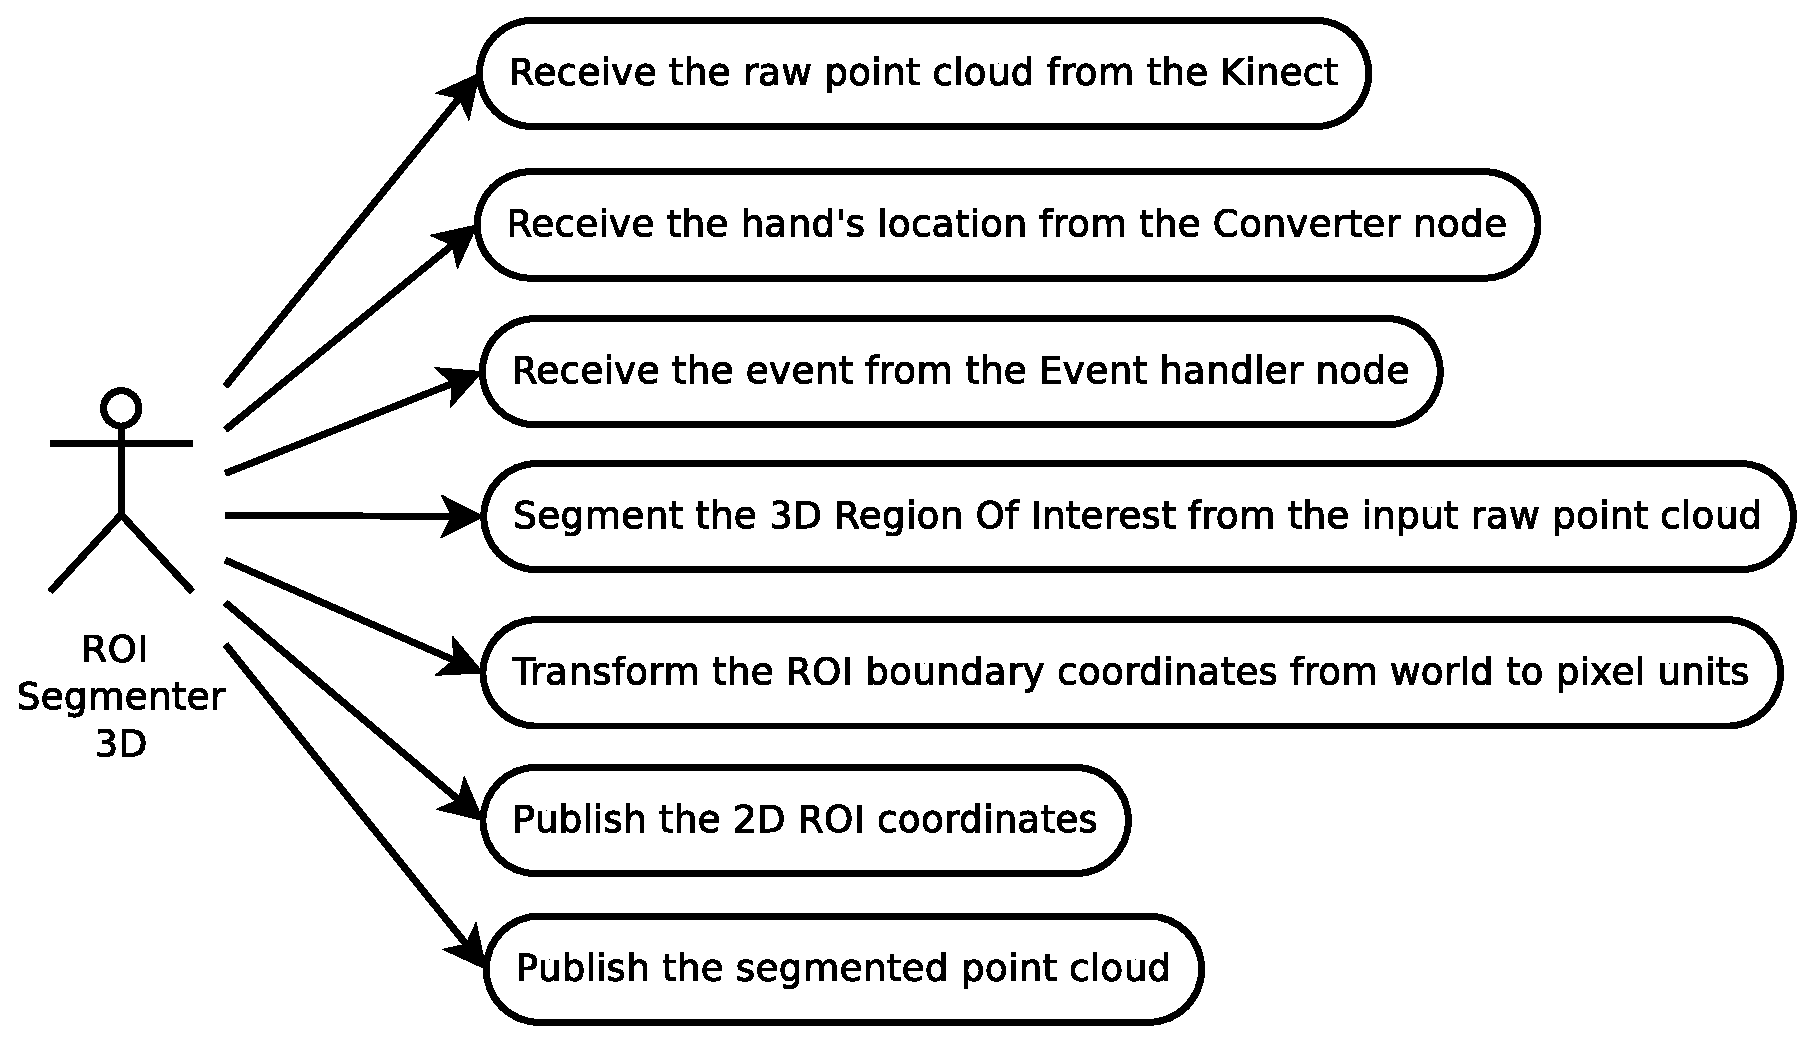
\includegraphics[scale=0.4]{img/diagrams/uc_roi_segmenter_3d.eps}
		\caption[Use case diagram ROI segmenter 3D node]{Use Case diagram of the ROI segmenter 3D node}
		
	\end{figure}
 
%\newpage

\paragraph{ROI Segmenter 2D}\mbox{}\\
	\label{roi_segmenter_2d}
	
	%The present node takes as the input the raw 2D information from the RGB-D sensor and the hand's locations in pixels returned from the ROI segmenter 3D node. 
	Figure \ref{node_roi2d} depicts the inputs and outputs of this node. 
	The raw 2D information and the hand location in pixels are inputs to the ROI Segmenter 2D node. 

		\begin{figure}[H]
			\begin{center}
			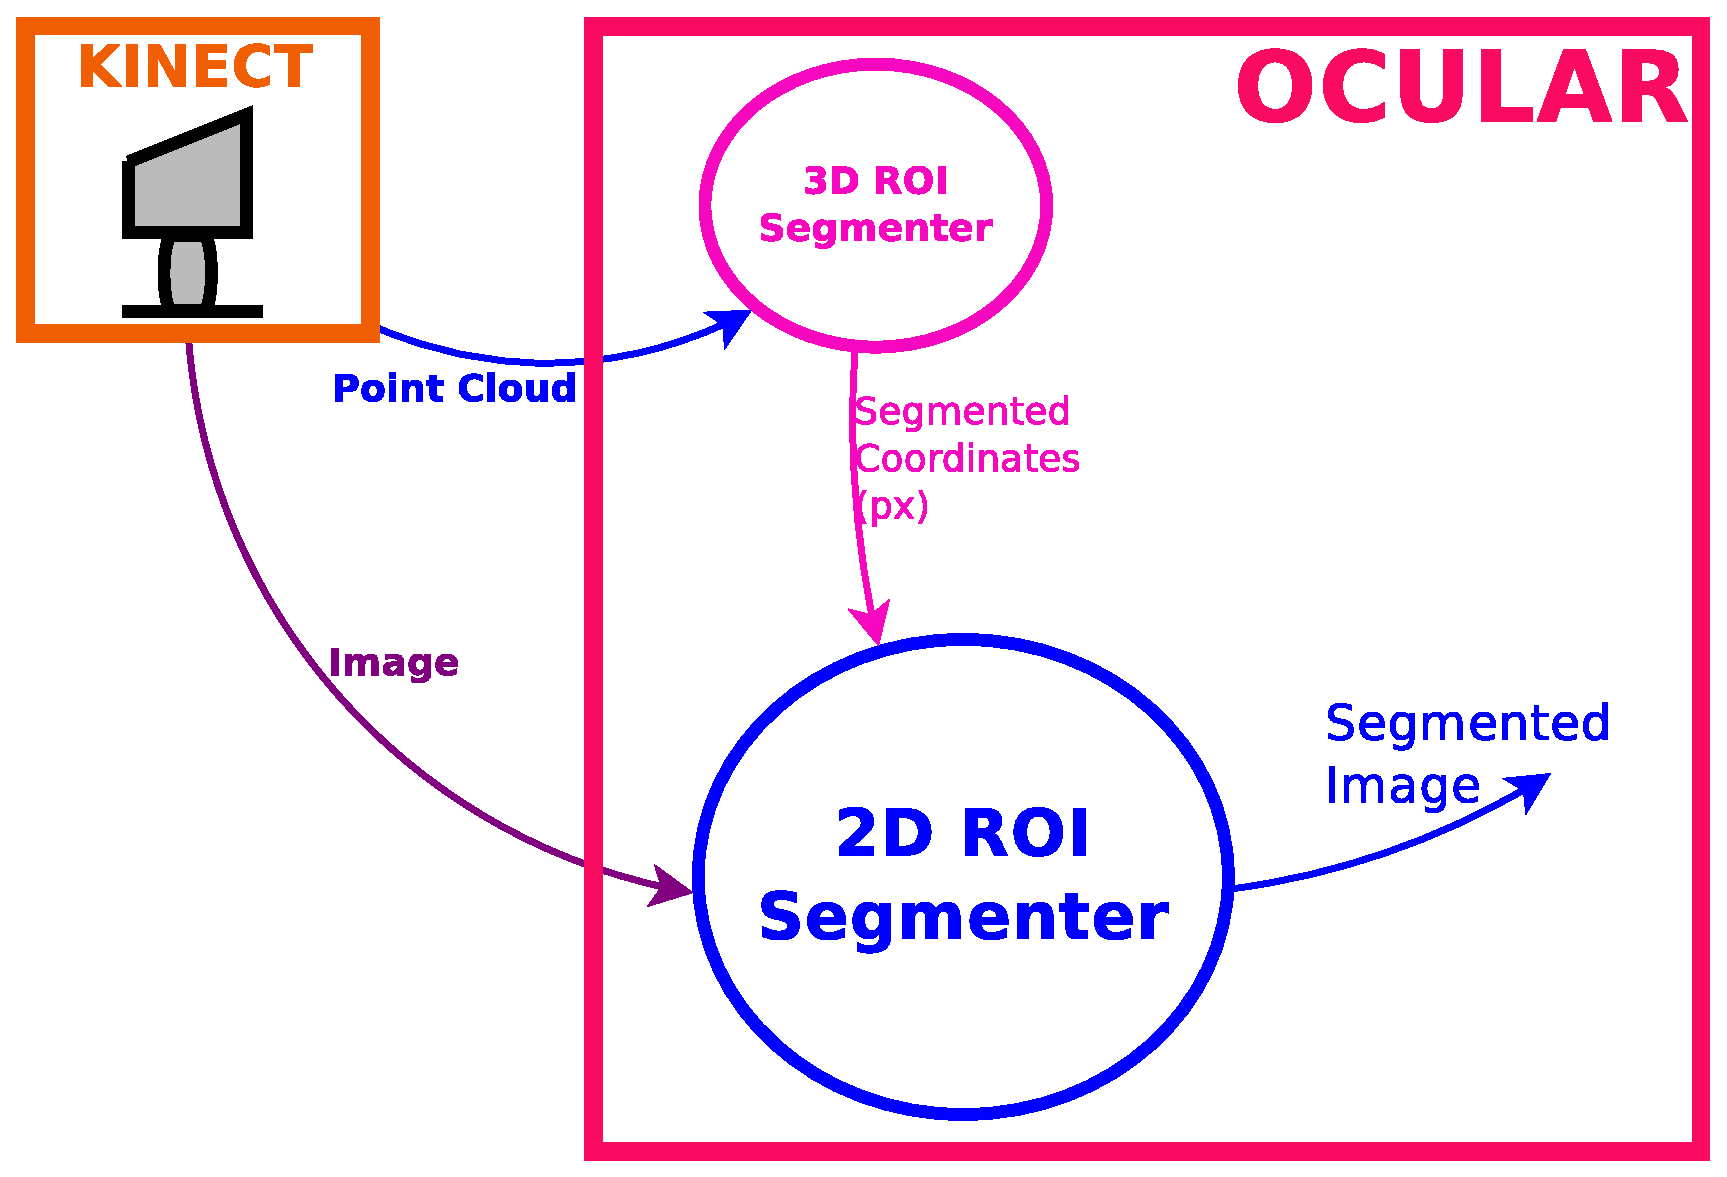
\includegraphics[width=0.5\linewidth]{img/diagrams/node_roi2d.eps}
			\caption[ROI segmenter 2D node I/O]{Inputs and outputs of the ROI segmenter 2D node.}		
			\label{node_roi2d}
			\end{center}
		\end{figure}

	The processing performed is the following: First, the ROI (Region Of Interest) is cropped taking a square section around the center of the hand. 
	The size of that figure is fixed for simplicity. 
	This fact does not affect the segmentation since the difference in the scale in negligible in the operating range of the system. 
	The range is determined by the skeleton tracker node and also the low resolution of the RGB-D sensor. 
	The system may be used at a distance between 1.5m and 2.5m. 
	%Since due to the RGB-D sensor's current resolutions the user must remain at a fixed distance from the sensor, the difference in the scale due to the distance is negligible and hence the size can be fixed. 
	\\
	In figure \ref{uc_roi2d} the use case diagram of the node can be observed.
	\begin{figure}[H]
		\centering
			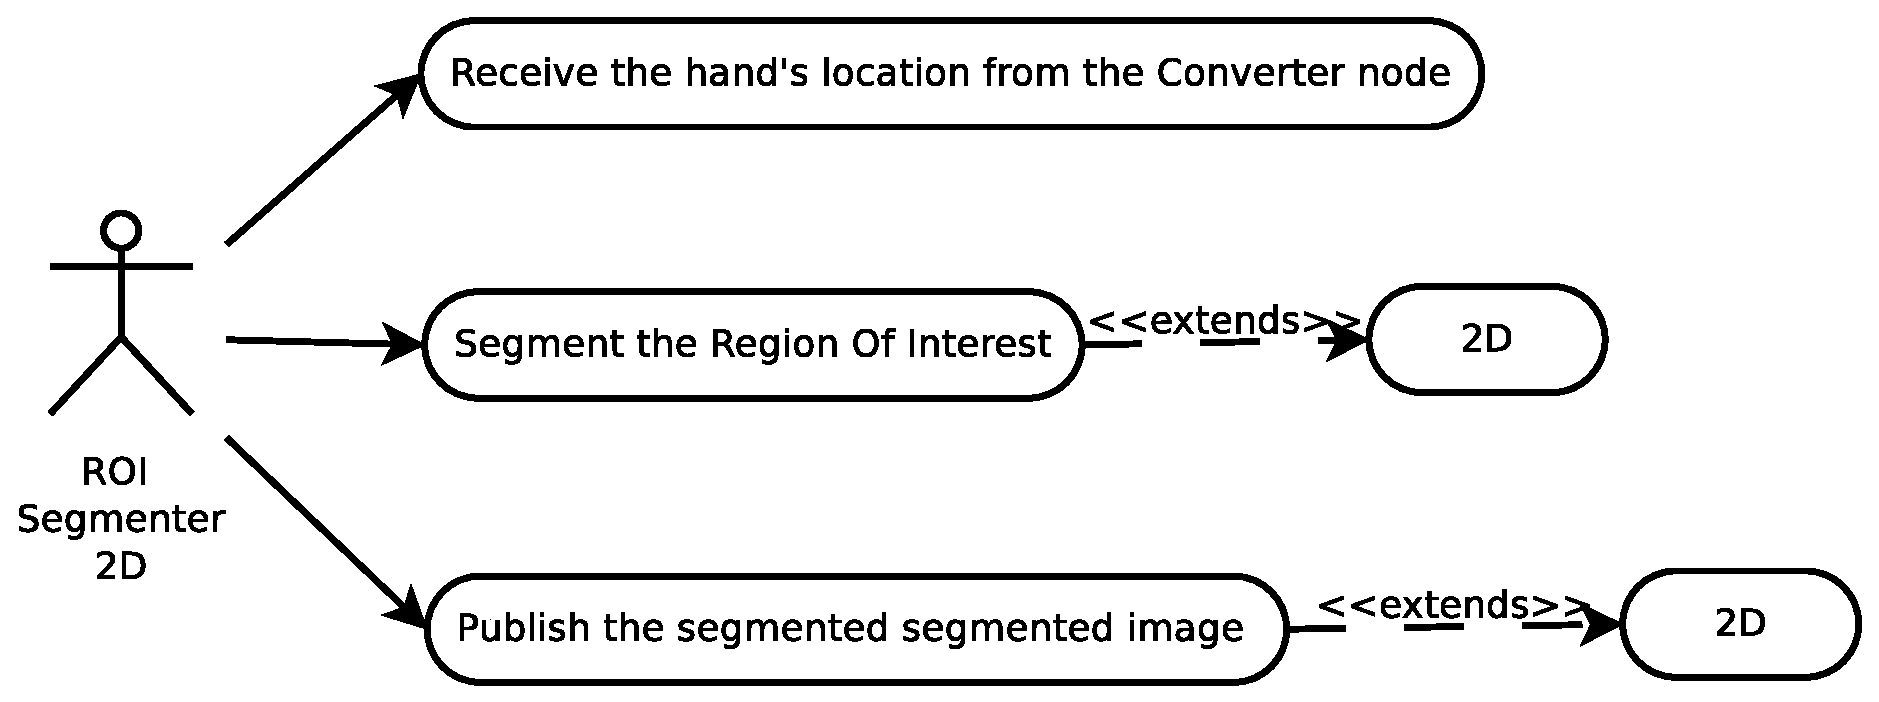
\includegraphics[scale=0.4]{img/diagrams/uc_roi_segmenter_2d.eps}
			\caption[Use case diagram ROI segmenter 2D node]{Use Case diagram of the ROI segmenter 2D node}
		\label{uc_roi2d}
	\end{figure}

%\newpage

\paragraph{Feature Extractor 2D}\mbox{}\\

	This node takes as an input the segmented 2D ROI from the previous nodes and extracts the features. 
	Figure \ref{node_fe2d} shows the inputs and outputs of the node. 

		\begin{figure}[H]
			\begin{center}
			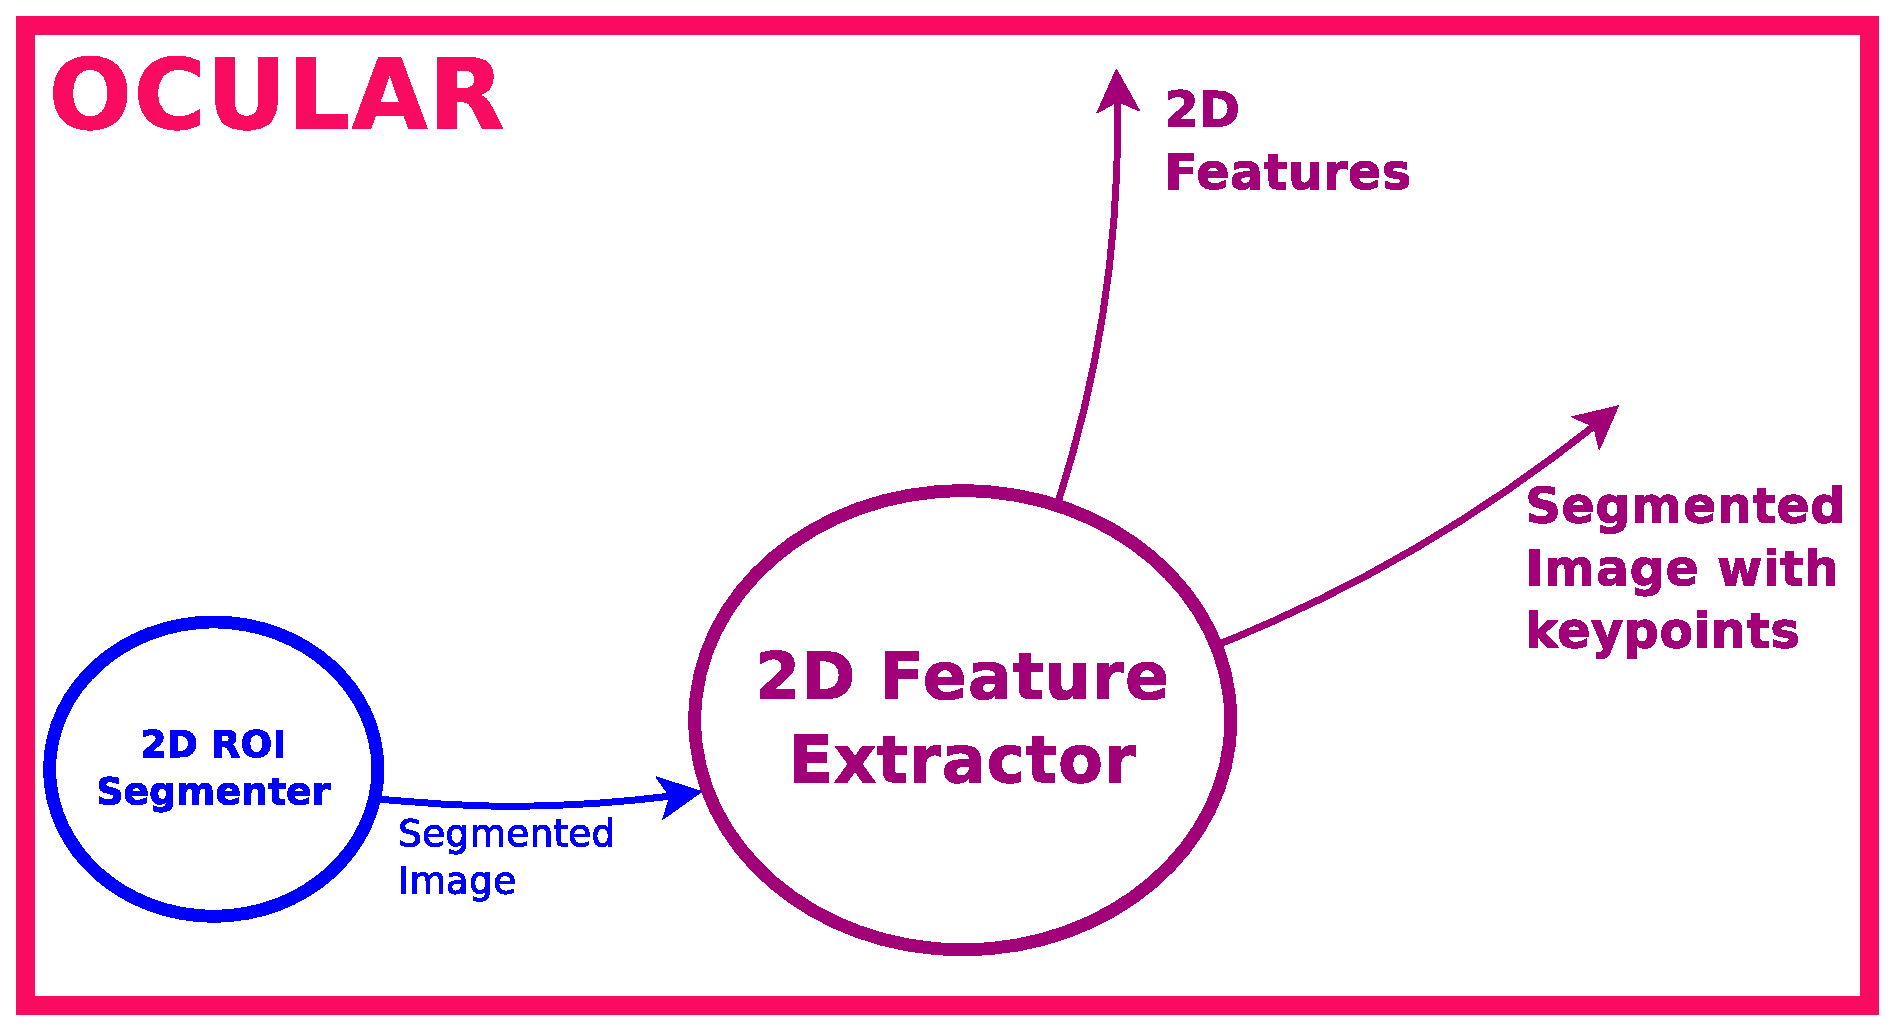
\includegraphics[width=0.5\linewidth]{img/diagrams/node_fe2d.eps}
			\caption[Feature Extractor 2D node I/O]{Inputs and outputs of the Feature Extractor 2D node.}		
			\label{node_fe2d}
			\end{center}
		\end{figure}

	There are two output messages of this node, the segmented images with keypoints and the 2D ORB descriptors. 
	The descriptors matrix is the one being used in the rest of the system. 
	The segmented image with the keypoints drawn on it is outputted for debugging and development reasons. 
	\\

	Figure  \ref{uc_fe2d} represents the use case diagram of this node. 
	\begin{figure}[H]
		\centering
			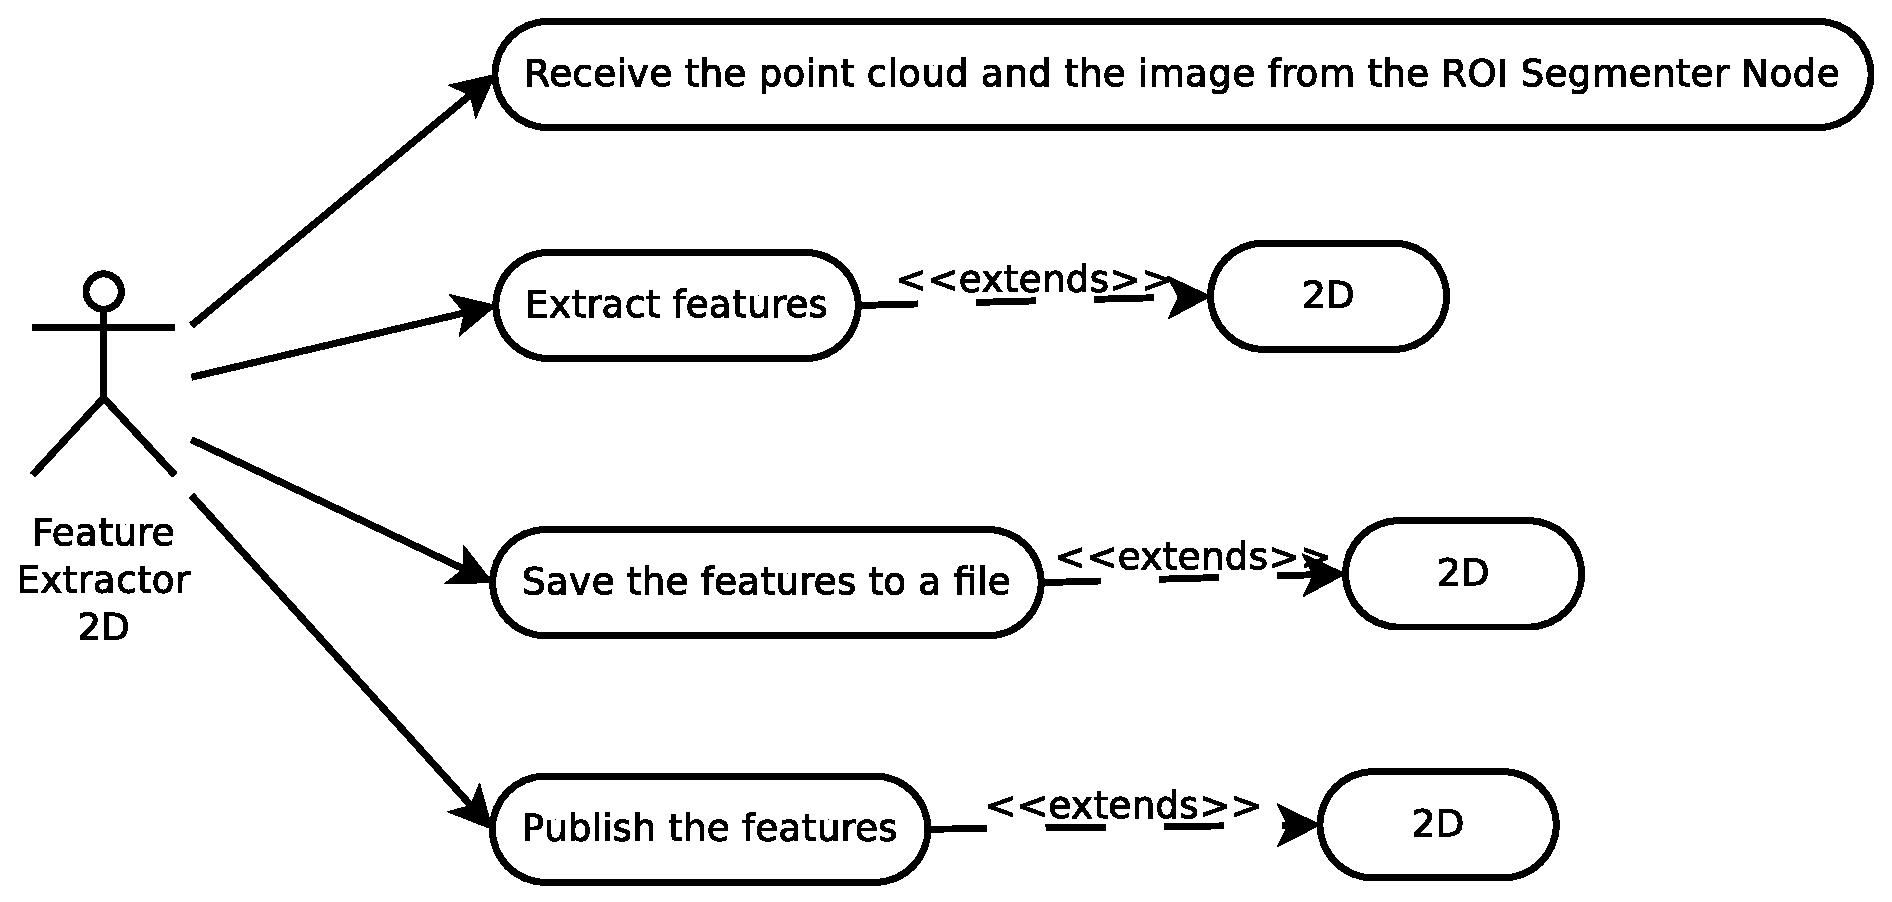
\includegraphics[scale=0.4]{img/diagrams/uc_feature_extractor_2d.eps}
			\caption[Use case diagram Feature Extractor 2D node]{Use Case diagram of the Feature Extractor 2D node}
		\label{uc_fe2d}
	\end{figure}

%\newpage

\paragraph{Feature Extractor 3D}\mbox{}\\

	The input of this node is the segmented point cloud from the ROI Segmenter 3D node. The descriptors are extracted from this information and are published in the output topic. 
	\\
		\begin{figure}[H]
			\begin{center}
			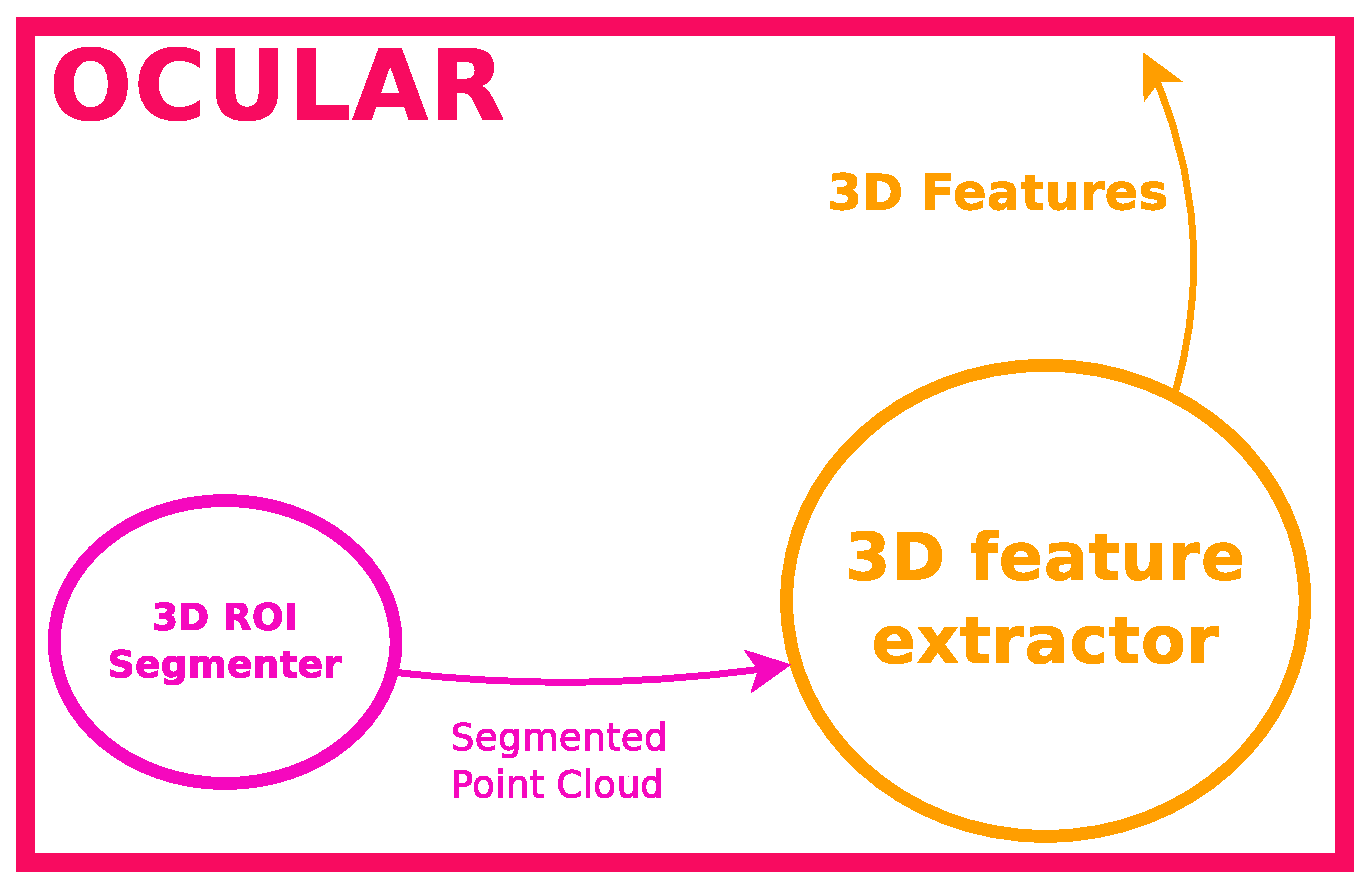
\includegraphics[width=0.5\linewidth]{img/diagrams/node_fe3d.eps}
			\caption[Feature Extractor 3D node I/O]{Inputs and outputs of the Feature Extractor 3D node.}		
			\label{node_fe3d}
			\end{center}
		\end{figure}

	The picture below shows the use case diagram of the node. 

	\begin{figure}[H]
		\centering
			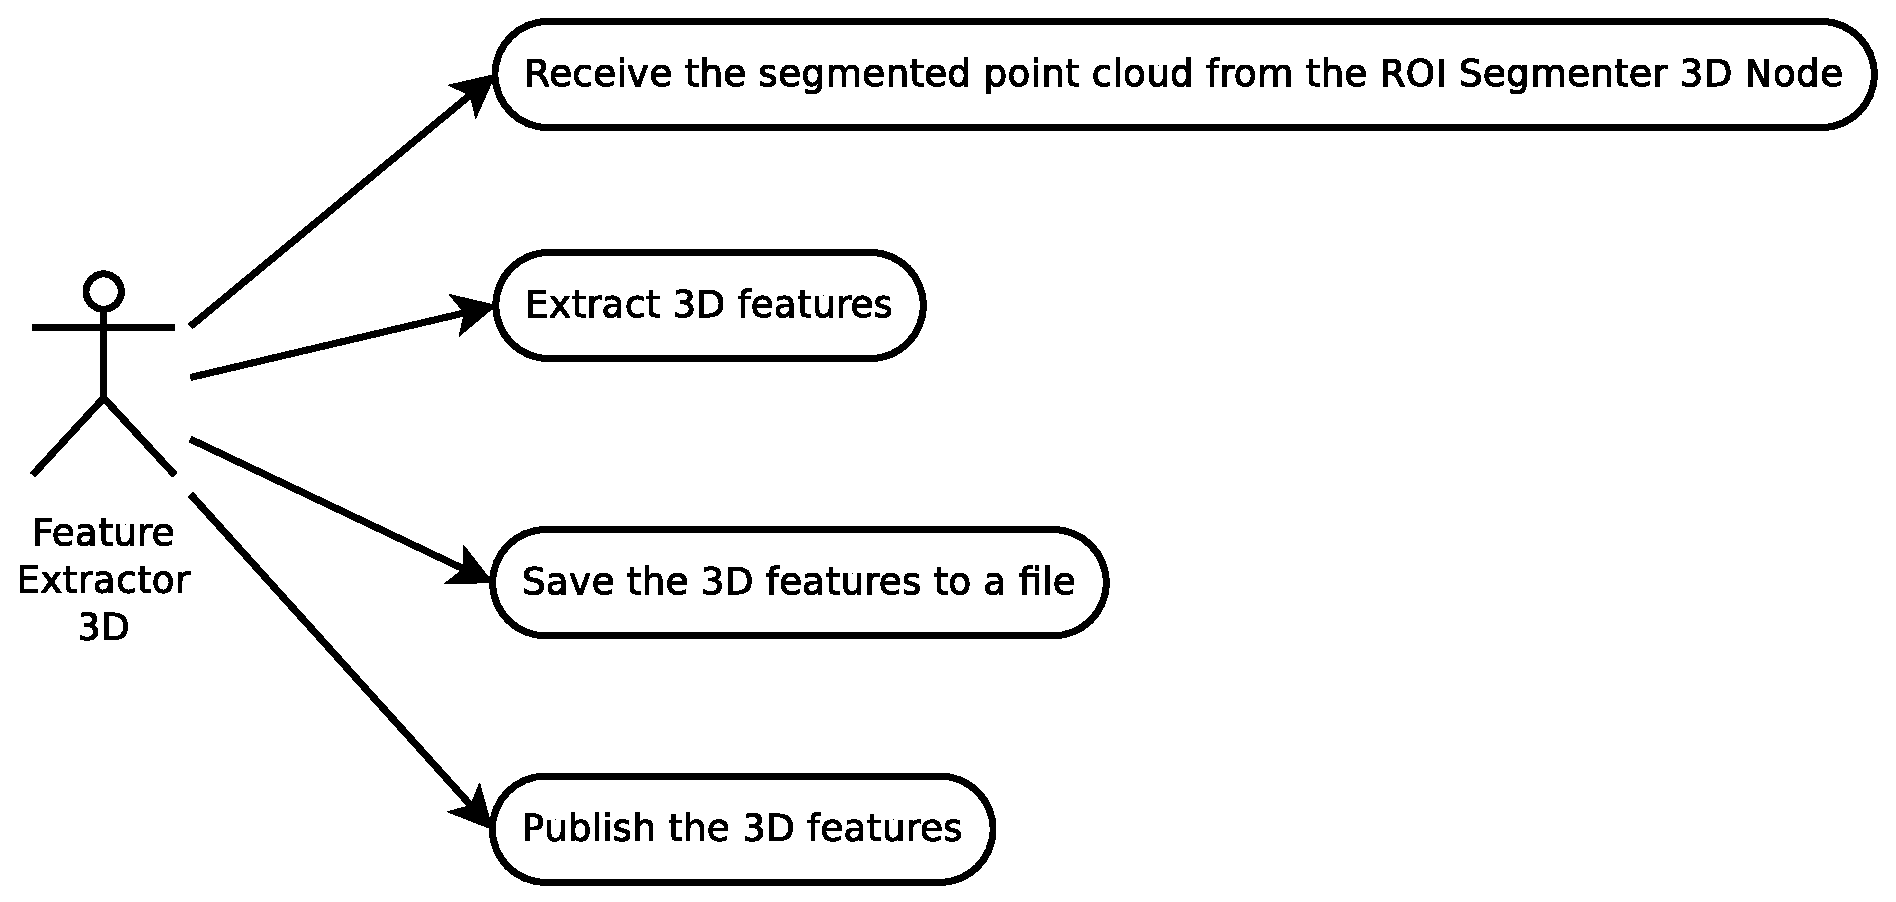
\includegraphics[scale=0.4]{img/diagrams/uc_feature_extractor_3d.eps}
			\caption[Use case diagram Feature Extractor 3D node]{Use Case diagram of the Feature Extractor 3D node}
		
	\end{figure}

%\newpage

\paragraph{Event Handler}\mbox{}\\

	As it was previously stated, in order to interact with the software some gestures were defined. This is the module that detects those gestures and switches accordingly to the corresponding event. This is the node responsible of detecting the different events that can appear in the system. 
	\\
	Figure \ref{node_event} shows the different inputs and outputs of the node. 
		\begin{figure}[H]
			\begin{center}
			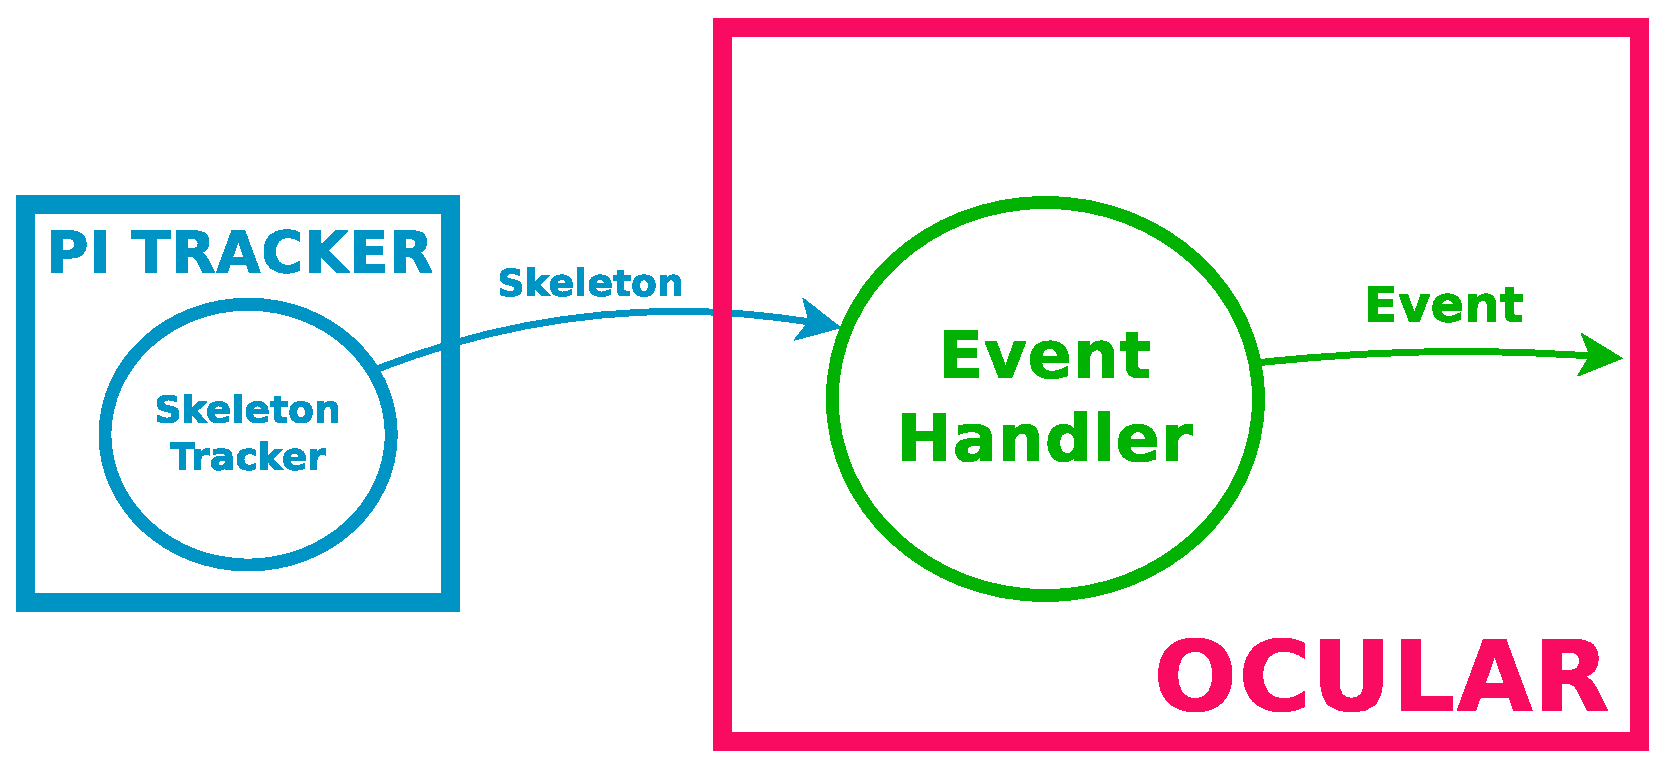
\includegraphics[width=0.5\linewidth]{img/diagrams/node_event.eps}
			\caption[Event Handler 3D node I/O]{Inputs and outputs of the Event Handler node.}		
			\label{node_event}
			\end{center}
		\end{figure}
	The input of the system is the skeleton message that is obtained from the third-party package pi\_tracker. This message contains the information of all the joints of the user. The information is screened to detect the height at which each hand is located. The one that is the highest is the one being used in the software. Afterwards, the distance between the body and the chosen hand is computed. When that distance is similar to the distance of the user's arm, the event triggered is "learn". If, otherwise, the hand is located close to the body, the event that is published to the output topic is "recognize". 
	\\

	The distance that triggers the modes is proportional to the distance between the user and the RGB-D sensor in order to obtain a range of use of the software higher. 
	Figure \ref{uc_event} is a diagram with the use case of the node. 
	\begin{figure}[H]
		\centering
			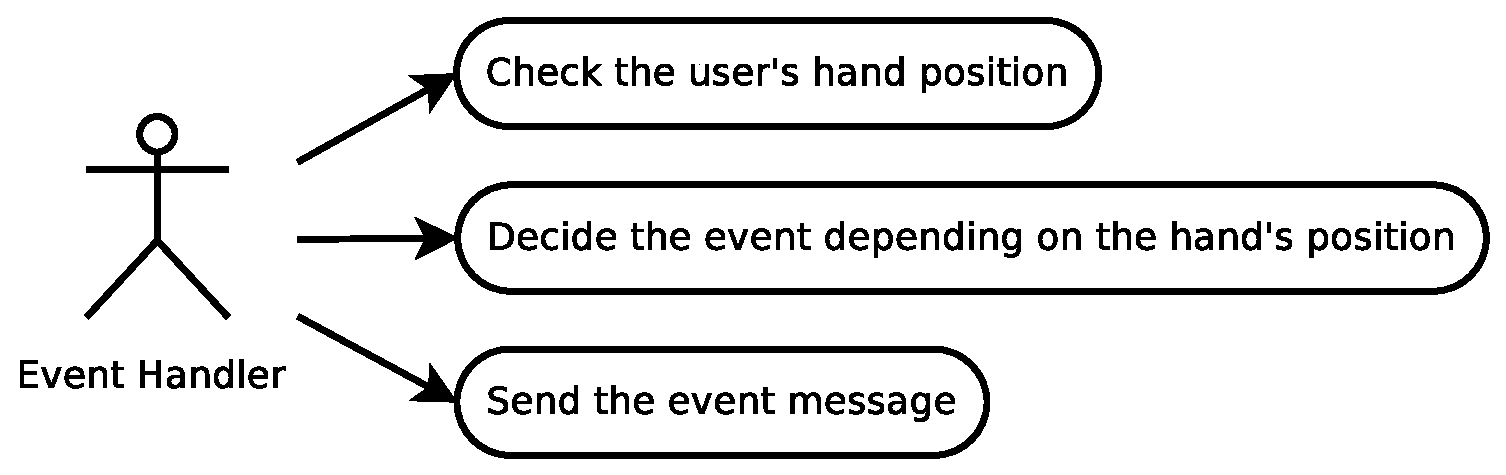
\includegraphics[scale=0.4]{img/diagrams/uc_event_handler.eps}
			\caption[Use case diagram Event Handler node]{Use Case diagram of the Event Handler node}
		\label{uc_event}
	\end{figure}

%\newpage

\paragraph{Learner Recognizer}\mbox{}\\
\label{learner_recognizer}

	This node implements the state machine depending on the events recognized by the event handler node. If the event received is "learn", the learning sequence starts. If the event is "recognize", the recognize sequence is triggered. 
	\\

		\begin{figure}[H]
			\begin{center}
			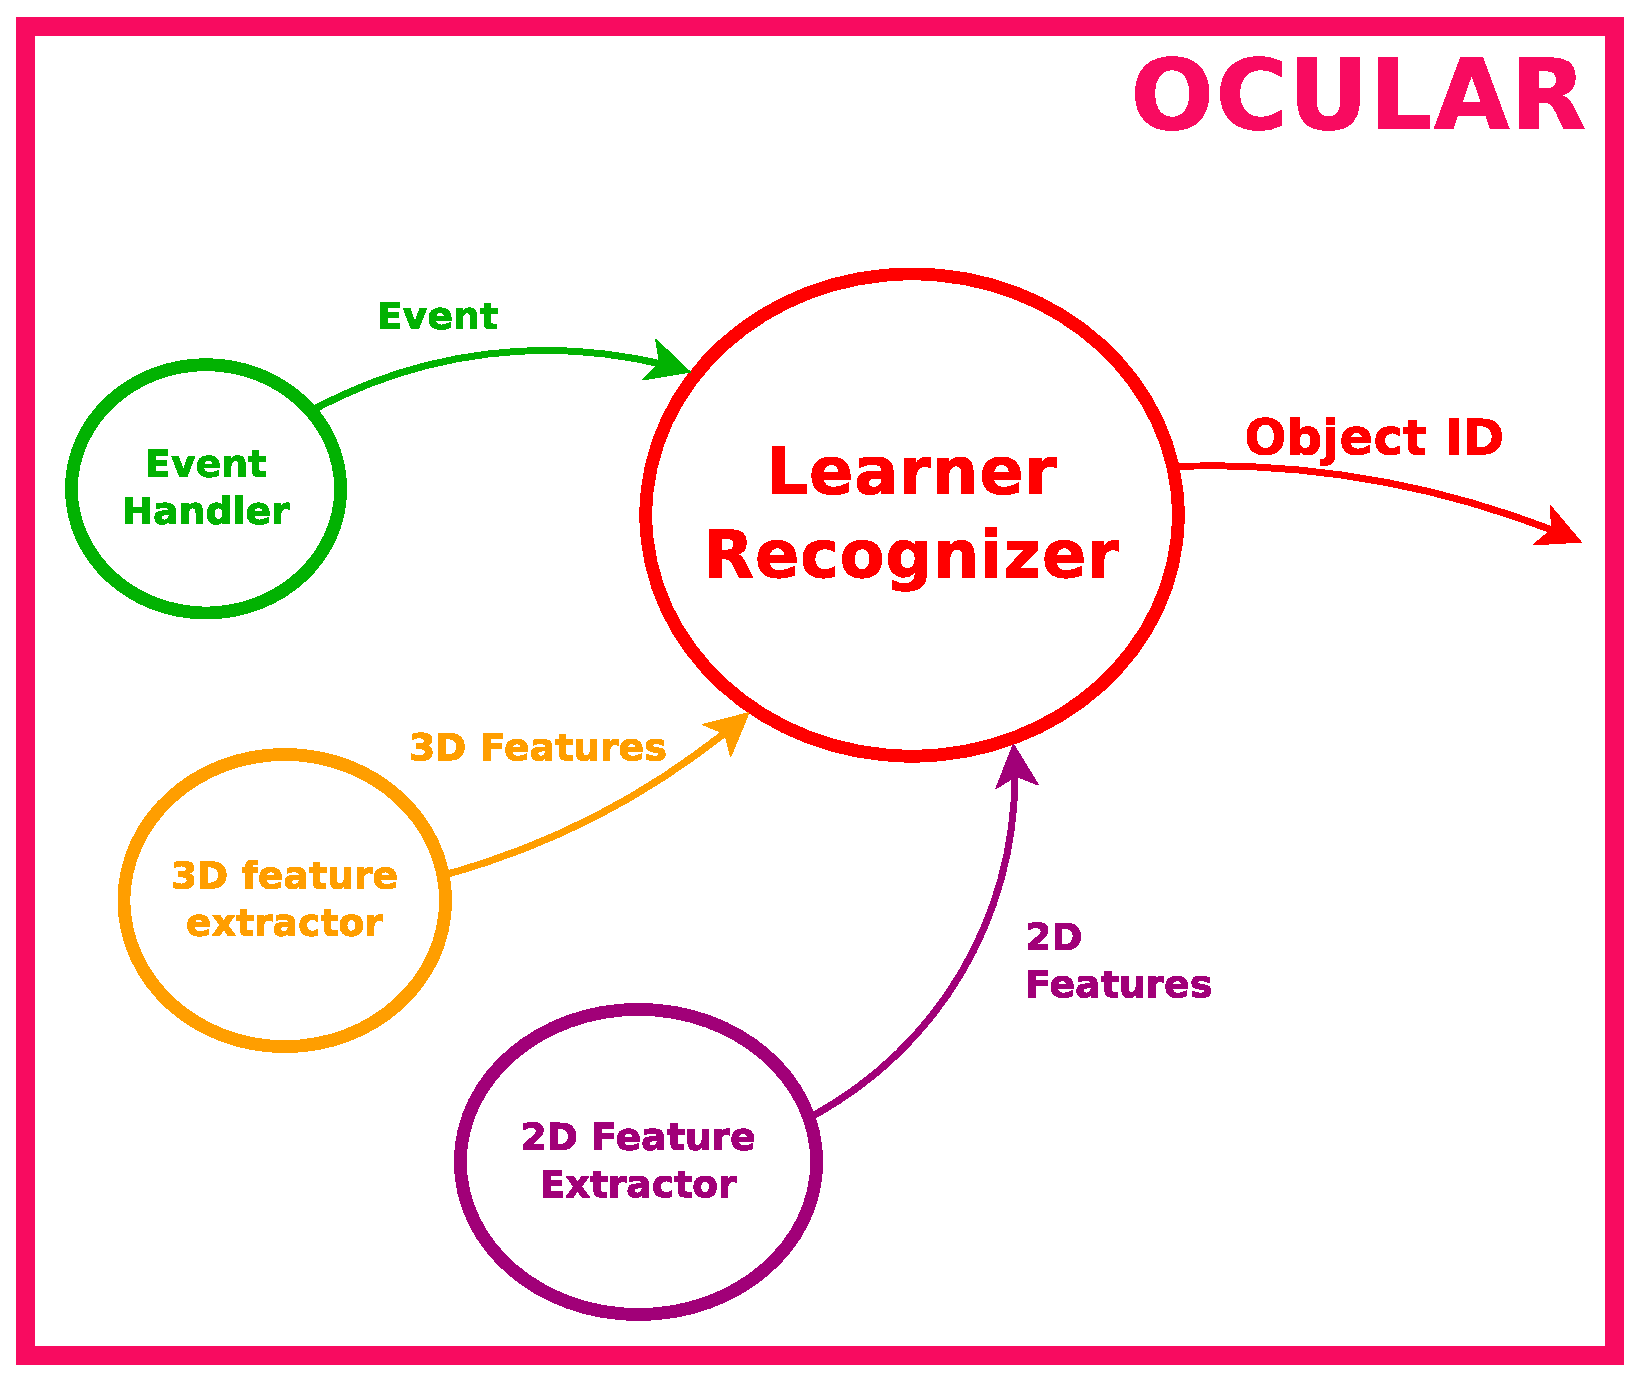
\includegraphics[width=0.5\linewidth]{img/diagrams/node_lr.eps}
			\caption[Learner Recognizer node I/O]{Inputs and outputs of the Learner Recognizer node.}		
			\label{node_lr}
			\end{center}
		\end{figure}

	The learn sequence consists on obtaining and storing the features both 2D and 3D and waiting a second allowing the user to move the object to capture a new view of it. 
	\\

	The recognition sequence compares the newly obtained features both 2D and 3D with the ones that are stored in the dataset. 
	Afterwards, the result of the recognition for both types of descriptors are published in the output topic. 
	Figure \ref{uc_learner_recognizer} presents the use case diagram of the node. 

	\begin{figure}[H]
		\centering
			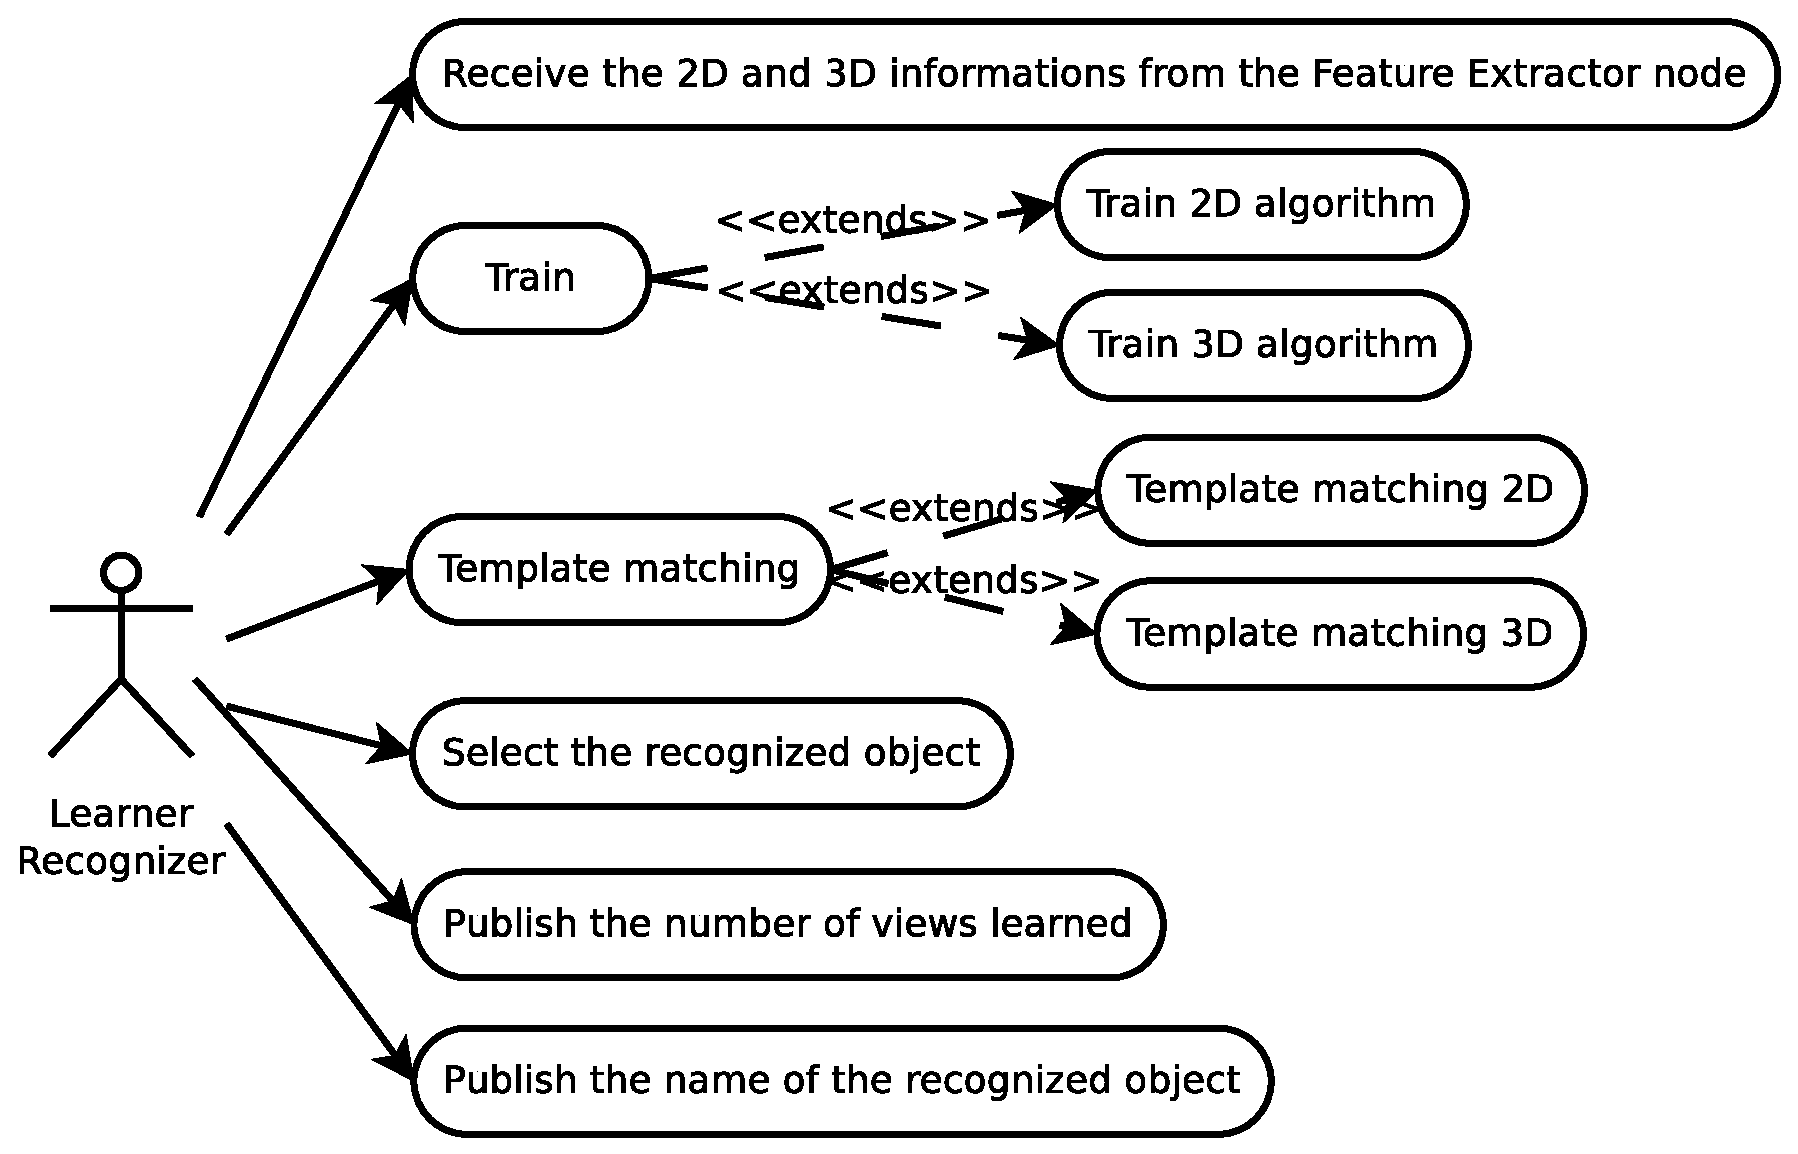
\includegraphics[scale=0.4]{img/diagrams/uc_learner_recognizer.eps}
			\caption[Use case diagram Learner Recognizer node]{Use Case diagram of the Learner Recognizer node}
			\label{uc_learner_recognizer}
	\end{figure}

%\newpage


\paragraph{System Output}\mbox{}\\

	This nodes implements a buffer and a decision algorithm. 
	The input of the node is the object ID message from the Learner Recognizer process as can be seen in figure \ref{node_output}.
	The node stores thirty values of instantaneous object estimations. 
	Since the Kinect runs at 30 frames per second, each second a new final object estimation appears. 
	The output of the node is the final object ID. 


		\begin{figure}[H]
			\begin{center}
			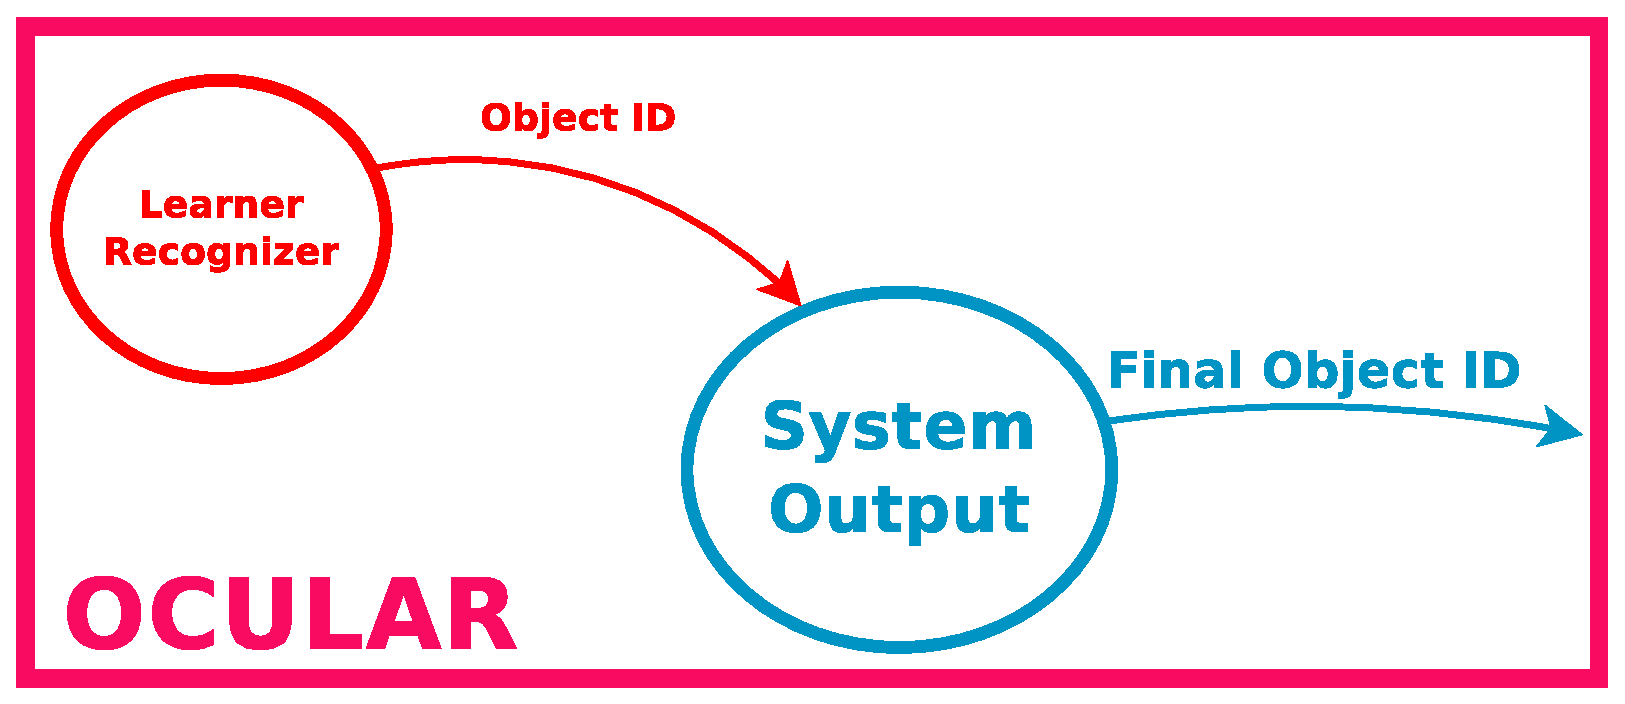
\includegraphics[width=0.5\linewidth]{img/diagrams/node_output.eps}
			\caption[System Output node I/O]{Inputs and outputs of the System Output node.}		
			\label{node_output}
			\end{center}
		\end{figure}

	The decision is performed as follows. 
	The input to the algorithm are two vectors containing the 2D and 3D object estimations. 
	The frequency of each class is obtained. 
	Let us represent as $y'_{2D}$ and $y'_{3D}$ the vectors containing in each element the frequency of the object with $object_id = element$. 
	Both informations are combined in one vector called $y'$. 
	\\
	\begin{center}
	$y'=0.6*y'_{2D}+0.4*y'_{3D}$
	\end{center}
	More importance is being given to the 2D estimations since the 2D descriptors are more robust than the 3D ones. 
	The estimated final object id ($Y$) is obtained as the vector element that has the highest value. 
	\\
	\begin{center}
		$Y'= argmax(y')$
	\end{center} 
	This number $Y$ is the output of this whole system. 
	\\
	Figure \ref{uc_output} shows the use case diagram of this node. 

	\begin{figure}[H]
		\centering
			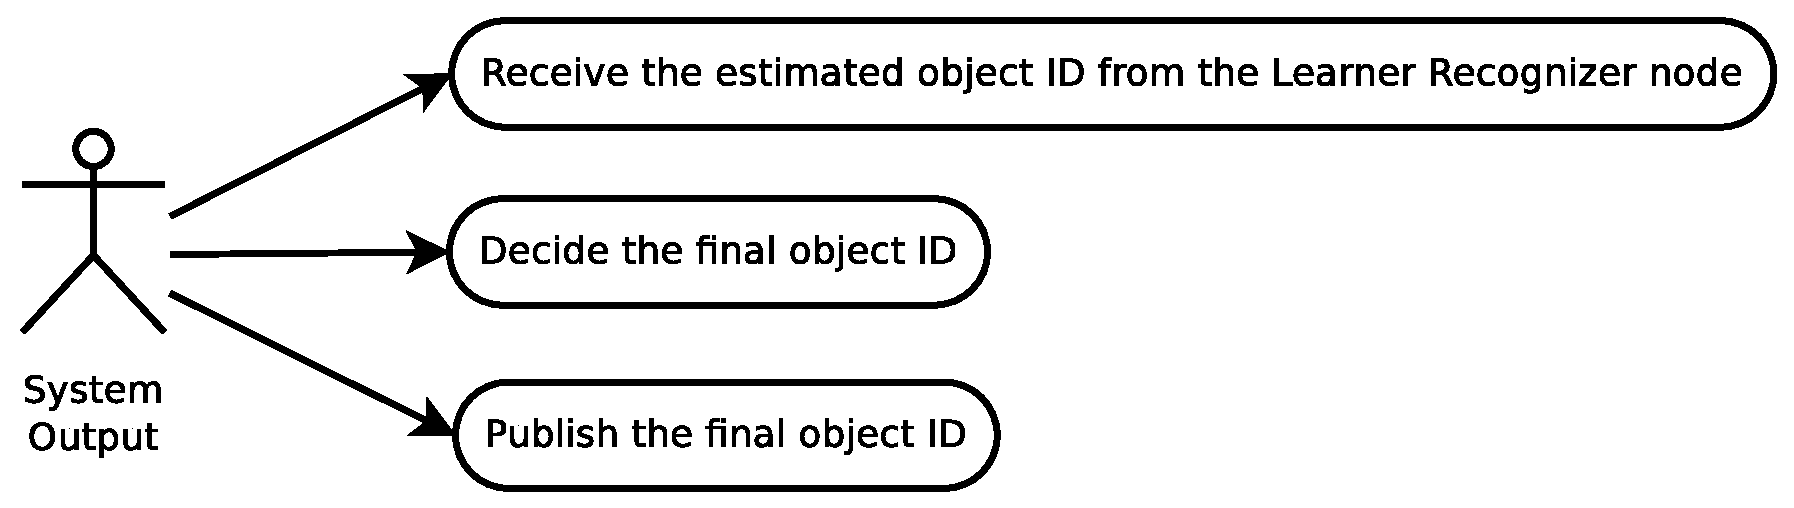
\includegraphics[scale=0.4]{img/diagrams/uc_system_output.eps}
			\caption[Use case diagram System Output node]{Use Case diagram of the System Output node}
			\label{uc_output}
	\end{figure}